\iffalse
\let\negmedspace\undefined
\let\negthickspace\undefined
\documentclass[journal,12pt,twocolumn]{IEEEtran}
\usepackage{cite}
\usepackage{amsmath,amssymb,amsfonts,amsthm}
\usepackage{algorithmic}
\usepackage{graphicx}
\usepackage{textcomp}
\usepackage{xcolor}
\usepackage{txfonts}
\usepackage{listings}
\usepackage{enumitem}
\usepackage{mathtools}
\usepackage{gensymb}
\usepackage{comment}
\usepackage[breaklinks=true]{hyperref}
\usepackage{tkz-euclide} 
\usepackage{listings}
\usepackage{gvv}                                        
\def\inputGnumericTable{}                                 
\usepackage[latin1]{inputenc}                                
\usepackage{color}                                            
\usepackage{array}                                            
\usepackage{longtable}                                       
\usepackage{calc}                                             
\usepackage{multirow}                                         
\usepackage{hhline}                                           
\usepackage{ifthen}                                           
\usepackage{lscape}

\newtheorem{theorem}{Theorem}[section]
\newtheorem{problem}{Problem}
\newtheorem{proposition}{Proposition}[section]
\newtheorem{lemma}{Lemma}[section]
\newtheorem{corollary}[theorem]{Corollary}
\newtheorem{example}{Example}[section]
\newtheorem{definition}[problem]{Definition}
\newcommand{\BEQA}{\begin{eqnarray}}
\newcommand{\EEQA}{\end{eqnarray}}
\newcommand{\define}{\stackrel{\triangle}{=}}
\theoremstyle{remark}
\newtheorem{rem}{Remark}

\graphicspath{{./figs/}}

\begin{document}

\bibliographystyle{IEEEtran}
\vspace{3cm}

\Large\title{NCERT Question 11.9.3.15}
\large\author{EE23BTECH11032 - Kaustubh Parag Khachane $^{*}$% <-this % stops a space
}
\maketitle
\newpage
\bigskip

\renewcommand{\thefigure}{\theenumi}
\renewcommand{\thetable}{\theenumi}
\large\textbf{Question 11.9.3.15} :

Given a GP with a = 729 and $7^{th}$ term 64, find $S_7$.

\solution
\fi
\begin{table}[ht] 
\centering
\setlength{\extrarowheight}{8pt}
\begin{tabular}{|l|l|l|}
    \hline
    \textbf{Parameter} & \textbf{Description} & \textbf{Value} \\
    \hline
     x\brak{0} & First Term & 729 \\
    \hline
     r & Common Ratio & \\
    \hline
      x\brak{n} & $\brak{n+1}^{th}$ Term & $x\brak{0}r^{n}u\brak{n}$ \\
    \hline
     x\brak{6} & $7^{th}$ Term & 64 \\
    \hline
    y\brak{k} & Sum of first \brak{k+1} terms & \\
    \hline
  \end{tabular}
  \vspace{4mm}
 \caption{Parameter Table}
 \label{tab:table0_11_9_3_15}
\end{table}


from \tabref{tab:table0_11_9_3_15} :
\begin{align}
    &x\brak{6} = x\brak{0}r^6\\
    \implies &64 = 729r^6\\
    &\therefore r = \frac{2}{3}\label{eq:eq2_11_9_3_15}
\end{align}
%using equation \eqref{eq:eq1} and equation \eqref{eq:eq2}
%\begin{align}
% s\brak{6} &= 729\frac{\brak{\frac{2}{3}}^6 - 1}{\frac{2}{3} - 1}\\
% & = \frac{729\left(\frac{2187 - 128}{2187}\right)}{\frac{1}{3}}\\
%\implies s\brak{6} &= 2059
%\end{align}
using \tabref{tab:table0_11_9_3_15} and equation \eqref{eq:eq2_11_9_3_15}
\begin{align}
    &X\brak{z} = \frac{729}{1 - \frac{2}{3}z^{-1}}\label{eq:eq6_11_9_3_15},\abs{z} > \frac{2}{3}
\end{align}
using \tabref{tab:table0_11_9_3_15} and equation \eqref{eq:eq6_11_9_3_15}
\begin{align}
    Y\brak{z} &= \frac{729}{\brak{1 - \frac{2}{3}z^{-1}}\brak{1-z^{-1}}}\\
    &= 2187\brak{\frac{1}{1-z^{-1}} - \frac{\frac{2}{3}}{1 - \frac{2}{3}z^{-1}}} \label{eq:eq5_11_9_3_15},\abs{z}  > 1
\end{align}
Using contour integration for inverse z transform,
\begin{align}
    y\brak{6} &= \frac{1}{2\pi j}\oint Y\brak{z} z^{5} dz \label{eq:eq12_11_9_3_15}
\end{align}
Using equation \eqref{eq:eq5_11_9_3_15} in \eqref{eq:eq12_11_9_3_15} :
\begin{align}
    y\brak{6}= \frac{1}{2\pi j}\brak{\oint\frac{2187z^{6}}{z-1}dz - \oint\frac{1458z^{6}}{z - \frac{2}{3}} dz} \label{eq:eq8_11_9_3_15}
\end{align}
\begin{align}
    \frac{1}{2\pi j}\brak{\oint\frac{2187z^{6}}{z - 1}dz} &= 2187\label{eq:eq9_11_9_3_15}\\
     \frac{1}{2\pi j}\brak{\oint\frac{1458z^{6}}{z - \frac{2}{3}}dz}  &= 128\label{eq:eq10_11_9_3_15}
     \end{align}
using equations \eqref{eq:eq9_11_9_3_15} and \eqref{eq:eq10_11_9_3_15} in \eqref{eq:eq8_11_9_3_15}:
\begin{align}
y\brak{6} &= 2187 - 128\\
&= 2059
\end{align}

\begin{figure}[!ht]
\centering
\begin{center}
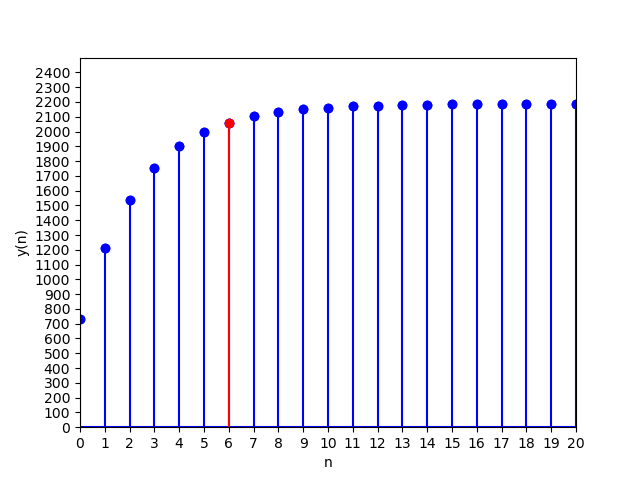
\includegraphics[width=\columnwidth]{ncert-maths/11/9/3/15/figs/Figure_1.png}
\end{center}
\caption{Plot of $y\brak{n}$}
\end{figure}
\begin{figure}[!ht]
\centering
\begin{center}
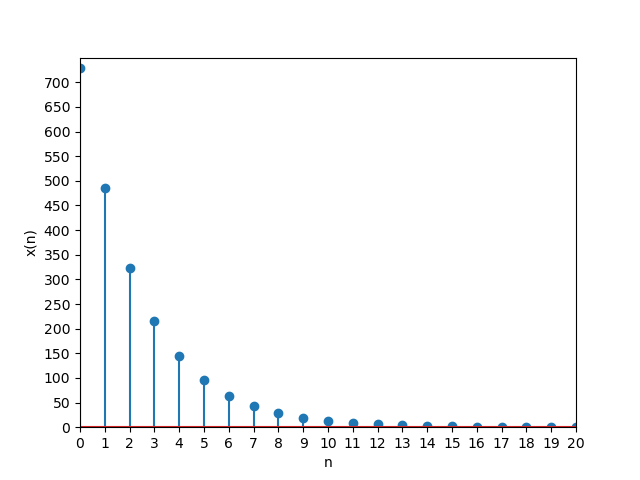
\includegraphics[width=\columnwidth]{ncert-maths/11/9/3/15/figs/Figure_2.png}
\end{center}
\caption{Plot of $x\brak{n}$}
\end{figure}
